% begin module piecewise-ex1
\begin{frame}
\begin{example}
Sketch the function $f(x)  = |2x-3|$.
\begin{columns}
\column{.4\textwidth}
\psset{xunit=1.6cm, yunit=1.6cm}
\begin{pspicture}(-0.5, -0.5)(2.8,2.8)
\tiny
\psframe*[linecolor=white](-0.5,-0.5)(2.8,2.8)
\psaxes{<->}(0,0)(-0.5,-0.5)(2.75,2.5)
\fcLabels{2.75}{2.5}
\uncover<6->{
\psline[linecolor=red](1.5, 0)(2.75,2.5)
}
\uncover<7->{
\psline[linecolor=red](0.25,2.5)(1.5, 0)
}
\end{pspicture}
%\only<-5| handout:0>{%
%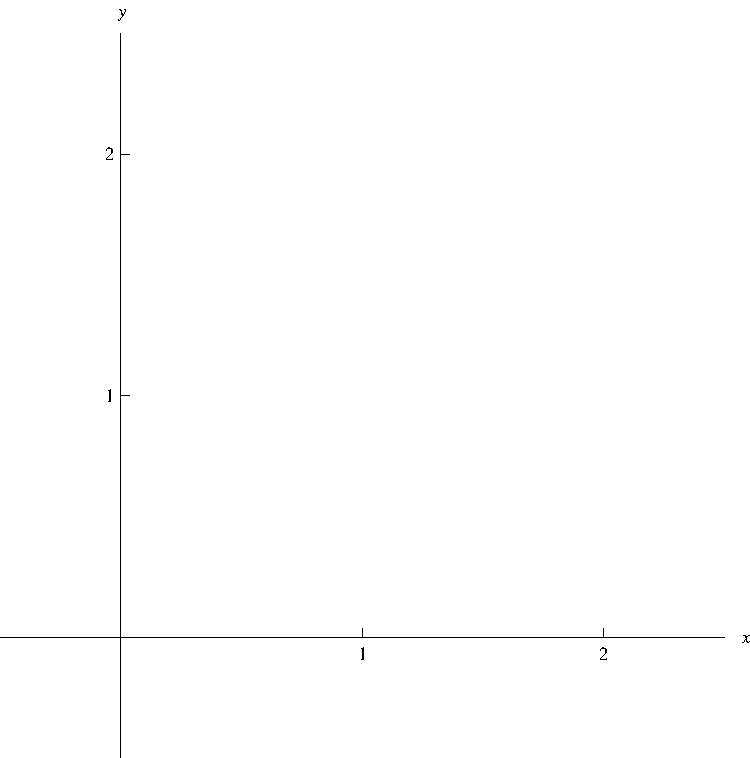
\includegraphics[width=4.5cm]{precalculus/pictures/piecewise-ex1-1.pdf}%
%}%
%\only<6| handout:0>{%
%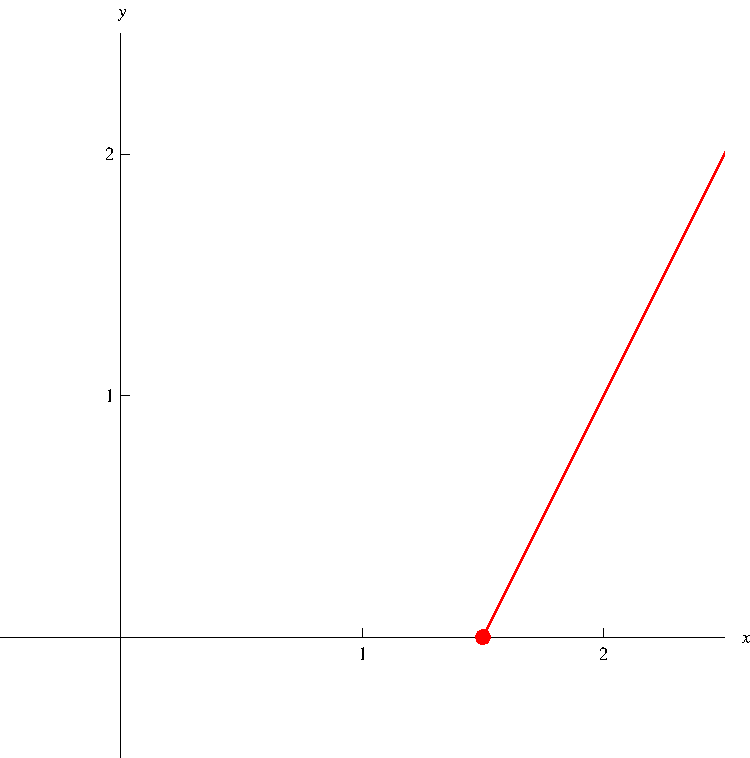
\includegraphics[width=4.5cm]{precalculus/pictures/piecewise-ex1-2.pdf}%
%}%
%\only<7-| handout:1>{%
%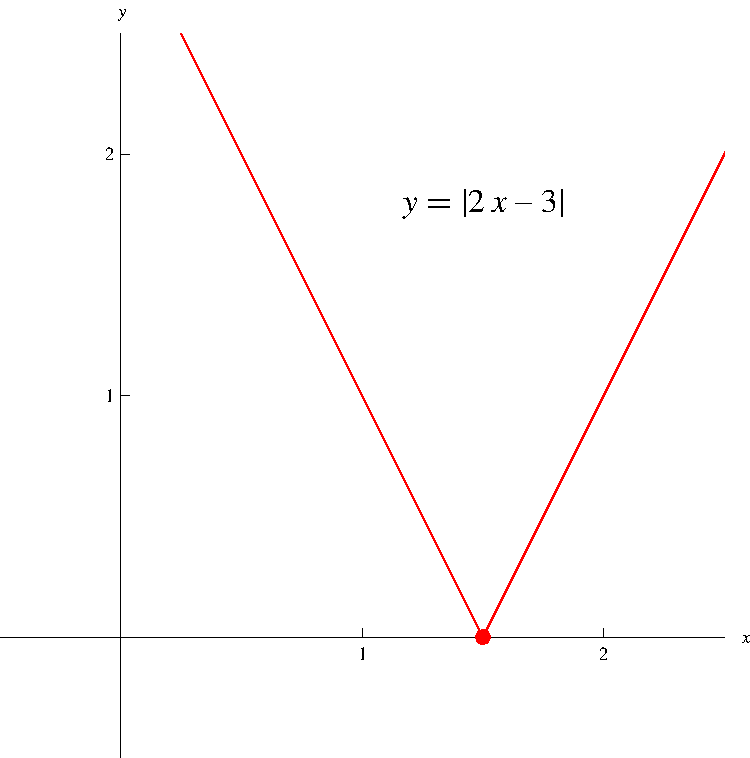
\includegraphics[width=4.5cm]{precalculus/pictures/piecewise-ex1-3.pdf}%
%}%
\column{.55\textwidth}
\abovedisplayskip=0pt
\belowdisplayskip=-15pt
\abovedisplayshortskip=0pt
\belowdisplayshortskip=0pt
\begin{align*}
\uncover<2->{%
|\alert<handout:0| 3>{x}| %
}%
& \uncover<2->{%
 = \begin{cases}
\alert<handout:0| 3>{x} & \text{if $\alert<handout:0| 3>{x} \geq 0$}\\
-\alert<handout:0| 3>{x} & \text{if $\alert<handout:0| 3>{x} < 0$}.\\
\end{cases}
}\\%
\uncover<3->{%
|\alert<handout:0| 3>{2x-3}| %
}%
& \uncover<3->{%
 = \begin{cases}
\alert<handout:0| 3>{2x-3} & \text{if $\alert<handout:0| 3>{2x-3} \geq 0$}\\
-(\alert<handout:0| 3>{2x-3}) & \text{if $\alert<handout:0| 3>{2x-3} < 0$}\\
\end{cases}
}\\%
& \uncover<4->{%
 = \begin{cases}
2x-3 & \text{if $2x \geq 3$}\\
-2x+3 & \text{if $2x < 3$}\\
\end{cases}
}\\%
& \uncover<5->{%
 = \begin{cases}
\alert<handout:0| 6>{2x-3} & \alert<handout:0| 6>{\text{if $x \geq 3/2$}}\\
\alert<handout:0| 7>{-2x+3} & \alert<handout:0| 7>{\text{if $x < 3/2$}}.\\
\end{cases}
}%
\end{align*}
\end{columns}
\end{example}
\end{frame}
% end module piecewise-ex1
